\section{Simulation Testbed}
\label{sec:exp}
\subsection{Architectural Platform}
Since PCM memory is as yet not commercially available, we
have taken recourse to a simulated hardware environment to
evaluate the impact of the PCM-conscious operators.  For this
purpose, we chose Multi2sim~\cite{multi2sim}, an open source
application-only\footnote{Simulates only the application layer without
the OS stack.} simulator that can model a multithreaded, multicore,
superscalar x86 CPU and an AMD Evergreen GPU. It has support for both
functional simulation and cycle-accurate detailed architecture simulation.

Since Multi2sim does not have native support for PCM, we modified its
existing DRAM module to mimic PCM behavior.  A separate architecture
controlled DRAM buffer was included as an additional level in the memory
hierarchy, specifically between the L2 cache and the PCM. The DRAM was
simulated as a set associative write-back memory with \textit{N-Chance}
as the eviction policy. As recommended in \cite{nchance}, $N$ was set
to $\frac{n}{2}$, where $n$ is the cache associativity, since this
setting provides good performance on multiple metrics -- writes, energy
and latency.  Finally, the timing simulation was modified to account
for the asymmetric read and write latencies of PCM.


\begin{comment}
Since our experiments consider J
In our experiments, we have used $n$ to be 8, therefore making $N$ to be 4.
\end{comment}

Like most other architectural simulators, Multi2Sim does not
explicitly track the data residing at the different levels of the
memory hierarchy. It instead maintains only a single buffer that
indicates the latest data, as visible to the simulated program, for
each memory location. We therefore had to add separate data tracking
functionality for the DRAM and PCM resident data. Since we follow
a \textit{read-before-write} policy for DRAM eviction, this addition
enabled us to read the original PCM resident data block and compare
it with the evicted DRAM block, thereby restricting the writes to only
where the data bits differed. In the experiments, we measure writes at
both \textit{bit} and \textit{word} granularities.

Apart from the raw number of writes, a critical related metric for PCM
algorithms is their wear distribution. We therefore instrumented the
Multi2sim code to track block level wear distribution information. To
achieve this, separate counters were created that tracked word (4B)
writes to each location during the query processing activity.

The specific configurations used in the memory hierarchy (L1 Data,
L1 Instruction, L2, DRAM Buffer, PCM) evaluated in our experiments are
enumerated in Table~\ref{table:setup}.  These values are scaled down
versions, wrt number of lines, of the hardware simulation parameters
used in \cite{wear} -- the reason for the scaling down is to ensure
that the simulator running times are not impractically long. However,
we have been careful to ensure that the \emph{ratios} between the sizes
of adjacent levels in the hierarchy are maintained as per the original
configurations in \cite{wear}.

Finally, despite the Multi2sim simulator having support for multiple
threads/processes, we restricted our experiments to a single process with
a single thread of execution. This choice ensured that the entire private
DRAM was available to the executing query. The effect of reduced DRAM
availability due to multiple programs running in parallel was \emph{inferred}
by conducting additional experiments with reduced DRAM sizes, and 
these results are also presented here.

\begin{center}
\begin{table}[htbp]
\caption{Experimental Setup}
\label{table:setup}
\begin{tabular}{p{3.0cm}p{5.0cm}}
\toprule
Simulator & Multi2Sim-4.2 with added support for PCM\\ \hline

L1D cache (private) & 32KB, 64B line, 4-way set-associative, 4 cycle latency, write-back, LRU replacement policy\\ \hline
L1I cache (private) & 32KB, 64B line, 4-way set-associative, 4 cycle latency, write-back, LRU replacement policy\\ \hline   
L2 cache (private) & 256KB, 64B line, 4-way set-associative, 11 cycle latency, write-back, LRU replacement policy\\ \hline

DRAM buffer (private) & 4MB, 256B line, 8-way set-associative, 200 cycle latency, write-back, N-Chance replacement policy (N = 4)\\ \hline

Main Memory & 2 GB PCM, 4KB page, 1024 cycle read latency (per 256B line), 64 cycle write latency (per 4B modified word)\\
\bottomrule
\end{tabular}
\end{table}
\end{center}


\subsection{Database and Queries}
%We used TPC-H (version 2.16.0) 1GB PCM-resident database for our experiments.
For the data, we used the default 1GB database generated by the TPC-H
benchmark.  This size is certainly small compared to the database sizes
typically encountered in modern applications -- however, we again chose
this reduced value to ensure viable simulation running times.

\begin{comment}
Notwithstanding, to ensure that our results were not skewed 
as an outcome,  we used scaled down versions of the hardware simulation parameters
from \cite{wear}, taking care to preserve the size ratios between adjacent
memory devices.
\end{comment}

For simulating our suite of database operators (\textit{sort},
\textit{hash join} and \textit{group by}), we created a separate
library consisting of the native PostgreSQL implementation of these
operators. To this library, we added the PCM-conscious versions described in
the previous sections.


While we experimented with several of the TPC-H queries, results for
three queries: Query 13 (Q13), Query 16 (Q16) and Query 19 (Q19), that
cover a diverse spectrum of the experimental space, are presented here.
For each of the queries, we first identified the query execution plan
recommended by the PostgreSQL query optimizer with the native operators,
and then forcibly used the same execution plan for their PCM-conscious
replacements as well. The SQL queries are show in Figure~\ref{fig:queries}. The specific plans used for these three queries
are shown in Figure~\ref{fig:plan_trees}.

   \lstset{width=\textwidth,
          %frame = single,
          escapechar=@,
          language=SQL,
          basicstyle=\scriptsize
          }

\newsavebox{\firstlisting}
\begin{lrbox}{\firstlisting}% Store first listing
\begin{lstlisting}
select c_count, count(*) as custdist
from ( select c_custkey, count(o_orderkey)
       from customer left outer join orders on 
       c_custkey = o_custkey and 
       o_comment not like '%pending%accounts%'
       group by c_custkey
      ) as c_orders (c_custkey, c_count)
group by c_count
order by custdist desc, c_count desc;
\end{lstlisting}
\end{lrbox}

\newsavebox{\secondlisting}
\begin{lrbox}{\secondlisting}% Store first listing
\begin{lstlisting}
select p_brand, p_type, p_size,
        count(distinct ps_suppkey) as supplier_cnt
from partsupp, part
where p_partkey = ps_partkey
        and p_brand <> 'Brand#35'
        and p_type not like 'ECONOMY BURNISHED%'
        and p_size in (14, 7, 21, 24, 35, 33, 2, 20)
        and ps_suppkey not in ( select s_suppkey
            from supplier
            where s_comment like '%Customer%Complaints%')
group by p_brand, p_type, p_size
order by supplier_cnt desc, p_brand, p_type, p_size;

\end{lstlisting}
\end{lrbox}

\newsavebox{\thirdlisting}
\begin{lrbox}{\thirdlisting}% Store first listing
\begin{lstlisting}
select sum(l_extendedprice* (1 - l_discount)) as revenue
from lineitem, part
where
 ( p_partkey = l_partkey and p_brand = 'Brand#23'
    and p_container in ('SM CASE', 'SM BOX', 'SM PACK', 'SM PKG')
    and l_quantity >= 5 and l_quantity <= 5 + 10
    and p_size between 1 and 5 and l_shipmode in ('AIR', 'AIR REG')
    and l_shipinstruct = 'DELIVER IN PERSON' )
or 
(  p_partkey = l_partkey and p_brand = 'Brand#15'
   and p_container in ('MED BAG', 'MED BOX', 'MED PKG', 'MED PACK')
   and l_quantity >= 14 and l_quantity <= 14 + 10
   and p_size between 1 and 10 and l_shipmode in ('AIR', 'AIR REG')
   and l_shipinstruct = 'DELIVER IN PERSON')
or 
( p_partkey = l_partkey and p_brand = 'Brand#44'
   and p_container in ('LG CASE', 'LG BOX', 'LG PACK', 'LG PKG')
   and l_quantity >= 28 and l_quantity <= 28 + 10
   and p_size between 1 and 15 and l_shipmode in ('AIR', 'AIR REG')
   and l_shipinstruct = 'DELIVER IN PERSON' );
\end{lstlisting}
\end{lrbox}

\begin{figure*}[ht]
\sbox{\measurebox}{
\begin{minipage}[b]{.33\textwidth}
\subfloat[Q13]{\usebox{\firstlisting}}
\hfill%
\subfloat[Q16]{\usebox{\secondlisting}}  
\end{minipage}
}
\usebox{\measurebox}\qquad
\hspace{4em}
\begin{minipage}[b][\ht\measurebox][s]{.33\textwidth}
\subfloat[Q19]{\usebox{\thirdlisting}} 
\end{minipage}
\caption{ Queries}

\label{fig:queries}
\end{figure*}





\subsection{Performance Metrics}
With regard to performance metrics, the number of PCM writes and the
running times (in terms of processor cycles) was measured for each of the
operators invoked during the query execution.  To enhance the accuracy
in the calculation of these metrics, a separate DRAM flushing routine
was inserted after the completion of each operator. This routine went
through the entire DRAM buffer, flushing out the previous entries,
leading to the number of writes being correctly estimated since all
dirty entries are evicted.

\begin{figure*}
\centering
\subfloat[Q13]{
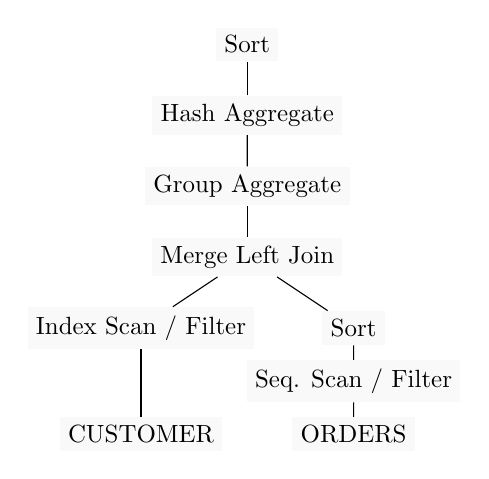
\begin{tikzpicture}[scale=.9, transform shape]

\tikzstyle{every node} = [rectangle, fill=gray!5]

\node (d) at (0,3) {Index Scan / Filter};
\node (c) at (0,1.5) {CUSTOMER};

\node (s) at (3,3) {Sort};
\node (p) at (3,2.25) {Seq. Scan / Filter};
\node (a) at (3,1.5) {ORDERS};

\node (e) at (1.5,4) {Merge Left Join};
\node (f) at (1.5,5)  {Group Aggregate};
\node (g) at (1.5,6)  {Hash Aggregate};
\node (h) at (1.5,7)  {Sort};


\draw[-] (c) -- (d);
\draw[-] (a) -- (p);
\draw[-] (d) -- (e);
\draw[-] (p) -- (s);
\draw[-] (s) -- (e);
\draw[-] (e) -- (f);

\draw[-] (f) -- (g);
\draw[-] (g) -- (h);

\end{tikzpicture}
}
\subfloat[Q16]{
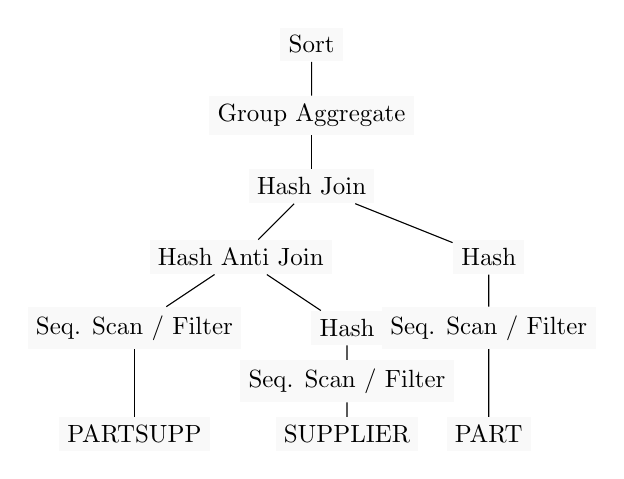
\begin{tikzpicture}[scale=.9, transform shape]

\tikzstyle{every node} = [rectangle, fill=gray!5]

\node (d) at (0,3) {Seq. Scan / Filter};
\node (c) at (0,1.5) {PARTSUPP};

\node (s) at (3,3) {Hash};
\node (p) at (3,2.25) {Seq. Scan / Filter};
\node (a) at (3,1.5) {SUPPLIER};

\node (e) at (1.5,4) {Hash Anti Join};

\node (n) at (5, 4) {Hash};
\node (b) at (5,3) {Seq. Scan / Filter};
\node (x) at (5,1.5) {PART};

\node (f) at (2.5,5)  {Hash Join};
\node (g) at (2.5,6)  {Group Aggregate};
\node (h) at (2.5,7)  {Sort};


\draw[-] (c) -- (d);
\draw[-] (a) -- (p);
\draw[-] (d) -- (e);
\draw[-] (p) -- (s);
\draw[-] (s) -- (e);
\draw[-] (e) -- (f);

\draw[-] (x) -- (b);
\draw[-] (b) -- (n);
\draw[-] (n) -- (f);

\draw[-] (f) -- (g);
\draw[-] (g) -- (h);

\end{tikzpicture}

}
\subfloat[Q19]{


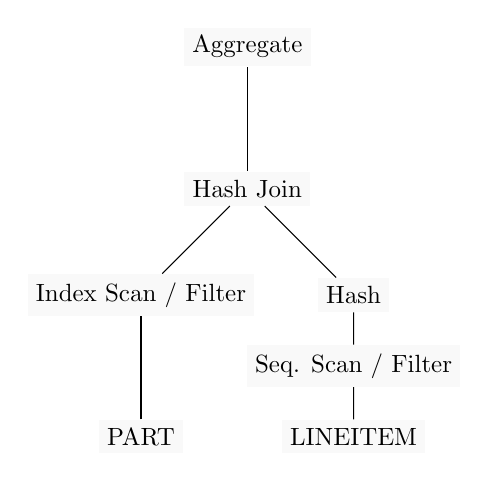
\begin{tikzpicture}[scale=.9, transform shape]

\tikzstyle{every node} = [rectangle, fill=gray!5]

\node (d) at (0,3.5) {Index Scan / Filter};
\node (c) at (0,1.5) {PART};

\node (s) at (3,3.5) {Hash};
\node (p) at (3,2.5) {Seq. Scan / Filter};
\node (a) at (3,1.5) {LINEITEM};

\node (e) at (1.5,5) {Hash Join};
\node (f) at (1.5,7)  {Aggregate};


\draw[-] (c) -- (d);
\draw[-] (a) -- (p);
\draw[-] (d) -- (e);
\draw[-] (p) -- (s);
\draw[-] (s) -- (e);
\draw[-] (e) -- (f);
\end{tikzpicture}
}

\caption{ Query plan trees}

\label{fig:plan_trees}

\end{figure*}
\section{Experimental Results}
\label{sec:results}


We conducted experiments based on the above framework and present
their results in this section. In particular, the PCM Writes and CPU Cycles results of the native
and PCM-conscious executions for Q13, Q15 and Q19 are shown in
Figures~\ref{fig:overall_results_q13}, \ref{fig:overall_results_q16}
and \ref{fig:overall_results_q19}, respectively.
In each of these figures, we provide both the total and the break-ups
on a per operator basis.

\begin{figure}[htbp]
  	\includegraphics[height=29mm]{overall_q13.png}
	\caption{Impact of sort on overall performance - Query 13}
	\label{fig:overall_results_q13}
\end{figure}
Focusing our attention first on Q13 in
Figure~\ref{fig:overall_results_q13}, we find that the bulk of the
overall Writes and Cycles are consumed by the Sort operator. Comparing
the performance of the Native (blue bar) and PCM-conscious (green bar)
implementations, we observe a very significant savings (57\%) on Writes,
and an appreciable decrease (22\%) on Cycles.

\begin{figure}[htbp]
	\centering
	\includegraphics[height=29mm]{overall_q16.png}
	\caption{Impact of group-by on overall performance - Query 16}
	\label{fig:overall_results_q16}
\end{figure}
Turning our attention to Q16 in Figure~\ref{fig:overall_results_q16},
we find that here, it is the group-by operator that primarily influences
the overall Writes performance, whereas the hash-join determines the
Cycles behavior. Again, there are substantial savings in both Writes
(40\%) and  Cycles (30\%) delivered by the PCM-conscious approach.

\begin{figure}[htbp]
	\centering
 	\includegraphics[height=29mm]{overall_q19.png}
	\caption{Impact of hash join on overall performance - Query 19}
	\label{fig:overall_results_q19}
\end{figure}



\begin{comment}
In case of Q13, the running time and writes for the sort operator formed
the bulk of the writes and time taken for the entire query. The group-by
operator comparatively incurred negligible writes and running time. Writes
savings of 84\% and running time savings of 42\% were observed for the
execution of Q13 (shown in sub-figures (a) and (b) resp.) as compared
to native; fuelled mainly by the sort operator.
\end{comment}



\begin{comment}
In case of Q16, both the group-by and hash join operators incurred
significant writes and time. We observed savings of $40\%$ in writes
besides $30\%$ savings in running time as compared to  native algorithms.
\end{comment}

Finally, moving on to Q19 in Figure~\ref{fig:overall_results_q19},
where hash-join is essentially the only operator, we find that the
savings are around $64\%$ with regard to Writes and $32\%$ in Cycles.

We now analyse the savings due to each operator independently, and
show their correspondence to the analysis in Sections~\ref{sort}--~\ref{gby} . 
 
\subsubsection{Sort}

\begin{comment}
The quicksort code from the GNU library was used for the conventional
version of sorting. On the other hand, the PCM-conscious version was
designed to employ a multi-pivot sort when the available DRAM was less
than the size of the data to be sorted; else, it reverted to the
native quicksort algorithm.
For Q13,  where the size of the ORDERS table is 216M, the write ratio
of native single-pivot quicksort to multi-pivot sort is estimated
by the bounds of Section~\ref{sort} to be within
$\displaystyle \frac{2}{2+ln\frac{N_R L_R}{|DRAM|} } \approx
\frac{2}{2+ln\frac {216M}{4M}  } \approx \frac{1}{3}$. These savings
are close to the $XX\%$ depicted by the ratio.
\end{comment}

\begin{comment}
the sort operator was the most heavily used and incurred
the majority of the writes and time. We observed a savings of about
70\% in writes and 20\% in running time. The size of orders table was
216M. 
\end{comment}
For Q13, we observed savings of $84\%$ in writes and $42\%$ in cycles. The PCM-conscious version used multi-pivot sort algorithm and incurred writes of $1.36 \times 10^6$ words $= 5.44 \times 10^6 $ bytes. The size of the $orders$ table was approximately $2.14 \times 10^6$. Replacing this value for $N_R L_R$ in Equation \ref{eq:mpivot}, we get the writes as $$W_{mpivot}(bytes) \approx 2 \times 2.14 \times 10^6  = 4.28 \times 10^6 $$ which is close to the observed writes.

In the case of Q16, however, the data at the sorting stage was found to be
much lesser than the DRAM size. Hence, both the native and PCM-conscious
executions used the native sort routine, and as a result, the cycles
and writes for both implementations match exactly.

\subsubsection{Hash Join}
Each entry in the hash table consisted of a pointer to the inner tuple
and a hash value field. New memory allocation to each bucket was done in
units of pages, with each page comprised of 64 entries. A search for the
matching join column(s) began with the first tuple in the corresponding
bucket and went on till the last tuple in that bucket, simultaneously
writing out join tuples for successful matches.

For Q16, we observed a $34\%$ improvement in Writes and $12\%$ in Cycles
due to the PCM-conscious hash join, as shown in Figure~\ref{fig:overall_results_q16}. 

These improvements were even higher
with Q19  -- 65\% Writes and 32\% Cycles in Figure~\ref{fig:overall_results_q19} -- the source of the enhancement
was the 3 bytes of writes saved due to single-byte hash values,
in addition to the page-based aggregation of hash table entries.

Using Equation \ref{eq:ht_pcm} for the estimated writes in Q19 for our PCM-conscious version of Hash Join and replacing the values of $N_R$, $size_{entry}$, $J$, $size_{hj}$ to be $2 \times 10^5$, $8$, $120$ and $8$, respectively, corresponding to Q16 at that stage, the writes are given by $$W_{ht\_pcm}(bytes) = 2 \times 10^5 (8-3) + 120 \times 8 \approx 10^6$$ which is close to the obtained writes of $0.32 \times 10^6$ words $= 1.28 \times 10^6$ bytes.
\subsubsection{Group By}

In Q16, the aggregate operator in the group-by has
an associated \textit{distinct} clause.  Thus, our group-by algorithm
utilized hash-based in-place partitioning followed by sorting to carry
out the aggregation. Both the partitioning and sorting were carried out
through pointers, thereby reducing the writes significantly. Consequently,
we obtain savings of $74\%$ in Writes and $20\%$ in Cycles, as shown in
Figure~\ref{fig:overall_results_q16}.

Equation \ref{eq:gby_ptr_hash} for write estimation in Pointer based hashed grouping algorithm depends upon $N_R$, $P$, $G$ and $size_g$. The values of these parameters for Q16 was $119056$, $4$, $18341$ and $48$ respectively. Replacing these values in the equation gives us 
$$W_{gb\_ptr\_hash}(bytes) = 2N_R \times P + G \times size_g$$
$$= 2 \times 119056\times 4 + 18341 \times 48$$ 
$$ = 1.83 \times 10^6$$ This closely corresponds to the observed writes of $0.36 \times 10^6$ words $= 1.44 \times 10^6$ bytes. 

When we consider Q13, however, the hash table consisted of very few entries. The lesser number of entries led to the overhead of page metadata itself overshadowing the savings obtained in other aspects. Specifically, improvements of
about 4\% and 1\% were obtained for Writes and Cycles, as shown in
Figure~\ref{fig:overall_results_q13}.

\begin{comment}

The data at this stage of the group-by was about 6 MB. Using the
bounds derived in Equations \ref{eq:gby_conv_sort} and \ref{eq:gby_ptr_hybrid}, the write ratios of the native and
PCM-conscious algorithms would be within $\frac{ \frac{2 \times size_{ptr}}{N_R
L_R} + 1}{2+ln\frac{N_R L_R}{|DRAM|} + 1} = \frac{1}{3+ln\frac {6M}{4M}
} \approx 29\%$, which is in accordance with the empirical savings of 74\%.

\end{comment}

\begin{figure*}[htbp]
\centering

\subfloat[Q13]{
  \includegraphics[width=5.8cm]{wear_q13.png}
}
\subfloat[Q16]{
  \includegraphics[width=5.8cm]{wear_q16.png}
}
\subfloat[Q19]{
  \includegraphics[width=5.8cm]{wear_q19.png}
}
\caption{Queries wear distribution }
\label{fig:wear_dist}
\end{figure*}



\subsection{Lifetime Analysis}
\begin{comment}
In \cite{qureshi}, the ideal lifetime $Y$ of a PCM device with size $S$
GB, $B$ write traffic, and cell endurance $W_{max}$, is given by:

$Y(years) = \frac{W_{max} \times S}{B} \times 2^{-25}$\\
\end{comment}

The above experiments have shown that PCM-conscious operators can
certainly provide substantive improvements in Writes and Cycles. However,
the question still remains as to whether these improvements have been
purchased at the expense of longevity of the memory. That is, are the
writes skewed towards particular memory locations?  To answer this, we
show in Figure~\ref{fig:wear_dist}, the maximum number of writes  across
all memory blocks (as mentioned earlier, we track writes at the block
level (256 bytes) in our modified simulator), for the three TPC-H queries. The x-axis displays the blocks numbers in decreasing order of writes.

We observe here that the maximum writes is considerably more for the
native systems as compared to the PCM-conscious processing. This
conclusively demonstrates that the improvement is with regard to
\emph{both} average case and worst case behavior.


\begin{comment}
Note that it is possible to achieve this lifetime only when the writes
are perfectly levelled across the entire PCM. In practice, however,
there is a degree of skewness in the writes of most algorithms. Due to
this skew, an algorithm might cut short the PCM lifetime considerably
despite doing well on the overall writes, since a particular set of
locations are written to repeatedly. Hence, characterizing the write
skew is fundamental to determining PCM durability.

As mentioned earlier, we track writes at the block level (256B) in our
modified simulator.  In Figure~\ref{fig:wear_dist}, we show the 
write frequencies of the top 100 blocks for the different operators.

As we can see, in the case of hash join, our PCM-conscious algorithms have
almost the same uniform distribution as the native algorithms. though the
initial part of the writes are slightly higher. This is in those cases
when the bitmap used for maintaining the slot occupancy information for
pages in the hash table is evicted intermediately between bit updates,
thereby incurring higher number of writes for that line.

For group-by (using sort), the per block writes due to our algorithms
are consistently lower than the native algorithms by about $39\%$. The
reason for this is that sorting incurs multiple writes for the same
block when all the input tuples cannot fit in DRAM, which the aspect of
partitioning saves in our PCM-conscious algorithms.

\begin{figure}[htbp]
	\psfig{figure=wear_dist.png, width = 9cm}\centering
	\caption{Operators Wear Distribution }
	\label{fig:wear_dist}
\end{figure} 
\end{comment}

\subsection{DRAM size sensitivity analysis}
We now move on to covering the scenario wherein the available DRAM
size at runtime is lesser than that anticipated prior to the query
execution -- for example, due to concurrent query processing. 
To model this scenario, we experiment with DRAM sizes of 512 KB, 1 MB and
2 MB. Note that, for each of these cases, all the algorithms continue to assume 4 MB as the available DRAM size, oblivious to the actual reduction in the availability of DRAM, and hence continue to execute accordingly. The results are shown in Figures~\ref{fig:sort}, \ref{fig:join}
and \ref{fig:gby} for the Sort, Hash Join and Group By operators, respectively.

\subsubsection{Sort}
In Figure~\ref{fig:sort}, we observe that the Sort operator provides average savings
for Q13 of about 50\% in Writes and 20\% in Cycles.

\begin{figure}[h]
	\centering
	\includegraphics[height=29mm]{sort_q13.png}
    \caption{Sort (Q13)}
	\label{fig:sort}
\end{figure}






%\subsubsection{Sort}

\begin{comment}
We omit sorting results for Q16. This is because our algorithm, being
oblivious to the change in the underlying DRAM size, chose to use the
native version of sort for all DRAM sizes since the data size was lesser
than the original DRAM size of 4MB.
\end{comment}

\subsubsection{Hash Join}
\begin{figure}[h]
	\centering
	\subfloat[Q16]{	
  	\includegraphics[height=29mm]{hj_q16.png}
	}
	\hspace{0mm}
	\subfloat[Q19]{
  	\includegraphics[height=29mm]{hj_q19.png}
	}
	\caption{Hash Join}
	\label{fig:join}
\end{figure}
In case of Q16, the hash join operator rendered $17\%$ improvement in
writes and $50\%$ in running time.

The hash join in Q19 continued to benefit with savings of about $42\%$ in writes and again $50\%$
in running time.

\begin{comment}
Not clear as to why the change in DRAM Size did not have any impact.
\end{comment}

\subsubsection{Group By} 
\begin{figure}[htbp]
\centering
\subfloat[Q13]{
  \includegraphics[height=29mm]{gb_q13.png}
}
\hspace{0mm}

\subfloat[Q16]{
  \includegraphics[height=29mm]{gb_q16.png}
}
\caption{Group By}
\label{fig:gby}
\end{figure}
The hash table being much smaller than all DRAM variants for Q13, the
change in the DRAM size didn't reflect much of a change in writes and
running time - yielding the same average of 4\% and 1\% for the two
metrics respectively.

For Q16, writes savings of $70\%$ and running time savings of $7\%$
were observed for the group-by operator.

Thus, we can conclude that the savings obtained by our algorithms are
not restricted to the environment where the DRAM is exclusively available
to one process. Instead, our algorithms can handle the unpredictability
in the DRAM availability due to multiple running processes equally well,
thereby being sufficiently robust to volatile system behaviour.


\subsection{Writes-Time Trade-off}
\label{tradeoff}
\begin{figure}[htbp]
	\centering
 	\includegraphics[height=29mm]{join_algos.png}
	\caption{Writes-Time trade-off in PCM algorithm design}
	\label{fig:join_algos}
\end{figure}
In this section, we present a sample query that characterizes the trade-off between writes and cycle time that in the design of algorithms for various operators. In the case of join operator, one such trade-off is observed in nested loops join and hash join. Consider, for example, the following modified TPC-H Query 16 :
\begin{verbatim}
select 
     p_brand, p_type, p_size,
     count(distinct ps_suppkey) 
     	as supplier_cnt
from 
     partsupp, part
where 
     p_partkey = ps_partkey
     and p_brand <> 'Brand#35'
     and p_type like 'ECONOMY BURNISHED%'
     and p_size in 
     	(14, 7, 21, 24, 35, 33, 2, 20)
     and ps_suppkey > 9950
group by 
     p_brand, p_type, p_size
order by 
     supplier_cnt desc, p_brand, 
     	p_type, p_size;
\end{verbatim}
We alternatingly used nested loops join and hash join to perform the join between $partsupp$ and $part$ tables. Figure \ref{fig:join_algos} presents the results for the two plans. Using nested loops join saves $65\%$ on writes as compared to hash join. On the other hand, hash join consumes a whopping $98\%$ lesser cycles than nested loops join by avoiding repeated iterations over the entire right table for every left table tuple. 

Hence, it is clear from the above example that future query optimizers for PCM based architecture need to incorporate these dual metrics of \emph{writes} and \emph{time} in order to decide the most suitable plan for executing a given query. 
\begin{comment}
\begin{table}[!h]
\centering
\caption{Overview of previous work on operators for PCM }
\label{tab:prev_work}
\begin{small}
\begin{tabular}{p{1.5cm}p{2.3cm}p{1.5cm}p{2cm}}
\toprule  
\textbf{Work} & \textbf{Model} &  \textbf{Operators} & \textbf{Write Guarantees}\\ 
\midrule
Chen et al. \cite{chen} & \textit{PCM\_DRAM} & B$^+$-tree, Hash Join & Hash join writes\\ \hline

Vamsikrishna et al. \cite{vamsi} & \textit {DRAM\_EXPLICIT} & Sort & Writes for basic version of PCM-aware sort\\ \hline

Viglas \cite{viglas} & \textit {DRAM\_EXPLICIT} & Sort, Join & Analysis of a subset of the algorithms presented based on some notion of relative read / write cost\\ 
\bottomrule
\end{tabular}
\end{small}
\end{table} 
\end{comment}
